% statistics_and_probability:x05 GDC:NO
\begin{question}
  \hspace*{\fill} [Note maximale: 14]\par
  \medskip
  \noindent Un sac A contient trois boules blanches et quatre boules rouges.\par
  \noindent Deux boules sont choisies au hazard et sans remise.\par
  \medskip
  (a)\par
  \hspace{1em} (i) Copiez et complétez le diagramme en arbre suivant. (N’écrivez rien sur cette page.)\par
  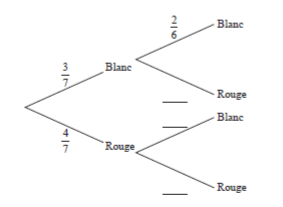
\includegraphics[scale=0.7]{arbre_rb}\par
  \hspace{1em} (ii) Trouvez la probabilité que deux boules blanches soient choisies.\hspace*{\fill} [5]\par
  \medskip  
  \noindent Un sac B contient quatre boules blanches et trois boules rouges. Quand deux boules sont choisies au hasard et sans remise dans le sac B, la probabilité qu’elles soient toutes les deux blanches est $\frac{2}{7}$\par
  \medskip
  \noindent Un dé standard est lancé. Si l’on obtient 1 ou 2, deux boules sont choisies au hasard et sans remise dans le sac A, sinon elles sont choisies dans le sac B.\par
  \medskip
  (b) Trouvez la probabilité que les deux boules soient blanches.\hspace*{\fill} [5]\par
  \medskip
  (c) Étant donné que les deux boules sont blanches,\par
  \hspace{2em} trouvez la probabilité qu’elles aient été choisies dans le sac A.\hspace*{\fill} [4]\par
  
  
\end{question}

